% !TEX root = main.tex
% !TEX root = main.tex
\documentclass[letterpaper, 11pt]{extarticle}
% \usepackage{fontspec}

% ==================================================

% document parameters
% \usepackage[spanish, mexico, es-lcroman]{babel}
\usepackage[english]{babel}
\usepackage[margin = 1in]{geometry}

% ==================================================

% Packages for math
\usepackage{mathrsfs}
\usepackage{amsfonts}
\usepackage{amsmath}
\usepackage{amsthm}
\usepackage{amssymb}
\usepackage{physics}
\usepackage{dsfont}
\usepackage{esint}

% ==================================================

% Packages for writing
\usepackage{enumerate}
\usepackage[shortlabels]{enumitem}
\usepackage{framed}
\usepackage{csquotes}

% ==================================================

% Miscellaneous packages
\usepackage{float}
\usepackage{tabularx}
\usepackage{xcolor}
\usepackage{multicol}
\usepackage{subcaption}
\usepackage{caption}
\captionsetup{format = hang, margin = 10pt, font = small, labelfont = bf}

% Citation
\usepackage[round, authoryear]{natbib}

% Hyperlinks setup
\usepackage{hyperref}
\definecolor{links}{rgb}{0.36,0.54,0.66}
\hypersetup{
   colorlinks = true,
    linkcolor = black,
     urlcolor = blue,
    citecolor = blue,
    filecolor = blue,
    pdfauthor = {Author},
     pdftitle = {Title},
   pdfsubject = {subject},
  pdfkeywords = {one, two},
  pdfproducer = {LaTeX},
   pdfcreator = {pdfLaTeX},
   }

% \begin{document}
% Hello, world! This is a minimal document to test the preamble.
% \end{document}

\usepackage{listings} 
\usepackage{xcolor}

\definecolor{codegreen}{rgb}{0.12,0.6,0.33}
\definecolor{codegray}{rgb}{0.5,0.5,0.5}
\definecolor{codepurple}{rgb}{0.58,0,0.82}
\definecolor{codeblue}{rgb}{0,0.1,0.8}
\definecolor{backcolour}{rgb}{0.95,0.95,0.92}

\lstdefinestyle{pythonstyle}{
   backgroundcolor=\color{backcolour},
   commentstyle=\color{codegreen},
   keywordstyle=\color{codeblue}\bfseries,
   numberstyle=\tiny\color{codegray},
   stringstyle=\color{codepurple},
   basicstyle=\ttfamily\footnotesize,
   breakatwhitespace=false,
   breaklines=true,
   captionpos=b,
   keepspaces=true,
   numbers=left,
   numbersep=5pt,
   showspaces=false,
   showstringspaces=false,
   showtabs=false,
   tabsize=4,
   language=Python
}

% \usepackage{minted}

\usepackage{titlesec}
\usepackage[many]{tcolorbox}

% Adjust spacing after the chapter title
\titlespacing*{\chapter}{0cm}{-2.0cm}{0.50cm}
\titlespacing*{\section}{0cm}{0.50cm}{0.25cm}

% Indent 
\setlength{\parindent}{0pt}
\setlength{\parskip}{1ex}

% --- Theorems, lemma, corollary, postulate, definition ---
% \numberwithin{equation}{section}

\newtcbtheorem[]{problem}{Problem}%
    {enhanced,
    colback = black!5, %white,
    colbacktitle = black!5,
    coltitle = black,
    boxrule = 0pt,
    frame hidden,
    borderline west = {0.5mm}{0.0mm}{black},
    fonttitle = \bfseries\sffamily,
    breakable,
    before skip = 3ex,
    after skip = 3ex
}{problem}

\tcbuselibrary{skins, breakable}

% --- You can define your own color box. Just copy the previous \newtcbtheorm definition and use the colors of yout liking and the title you want to use.
% --- Basic commands ---
%   Euler's constant
\newcommand{\eu}{\mathrm{e}}

%   Imaginary unit
\newcommand{\im}{\mathrm{i}}

%   Sexagesimal degree symbol
\newcommand{\grado}{\,^{\circ}}

% --- Comandos para álgebra lineal ---
% Matrix transpose
\newcommand{\transpose}[1]{{#1}^{\mathsf{T}}}

%%% Comandos para cálculo
%   Definite integral from -\infty to +\infty
\newcommand{\Int}{\int\limits_{-\infty}^{\infty}}

%   Indefinite integral
\newcommand{\rint}[2]{\int{#1}\dd{#2}}

%  Definite integral
\newcommand{\Rint}[4]{\int\limits_{#1}^{#2}{#3}\dd{#4}}

%   Dot product symbol (use the command \bigcdot)
\makeatletter
\newcommand*\bigcdot{\mathpalette\bigcdot@{.5}}
\newcommand*\bigcdot@[2]{\mathbin{\vcenter{\hbox{\scalebox{#2}{$\m@th#1\bullet$}}}}}
\makeatother

%   Hamiltonian
\newcommand{\Ham}{\hat{\mathcal{H}}}

%   Trace
\renewcommand{\Tr}{\mathrm{Tr}}

% Christoffel symbol of the second kind
\newcommand{\christoffelsecond}[4]{\dfrac{1}{2}g^{#3 #4}(\partial_{#1} g_{#2 #4} + \partial_{#2} g_{#1 #4} - \partial_{#4} g_{#1 #2})}

% Riemann curvature tensor
\newcommand{\riemanncurvature}[5]{\partial_{#3} \Gamma_{#4 #2}^{#1} - \partial_{#4} \Gamma_{#3 #2}^{#1} + \Gamma_{#3 #5}^{#1} \Gamma_{#4 #2}^{#5} - \Gamma_{#4 #5}^{#1} \Gamma_{#3 #2}^{#5}}

% Covariant Riemann curvature tensor
\newcommand{\covariantriemanncurvature}[5]{g_{#1 #5} R^{#5}{}_{#2 #3 #4}}

% Ricci tensor
\newcommand{\riccitensor}[5]{g_{#1 #5} R^{#5}{}_{#2 #3 #4}}

\begin{document}

\textsf{\LARGE{\textbf{Take-home exam 1}}}

\normalsize{\textit{Dynamical Systems}}

\vspace{1ex}

\textsf{\textbf{Student:}} \text{Males-Araujo Yorlan}, 
\href{mailto:yorlan.males@yachaytech.edu.ec}{\texttt{yorlan.males@yachaytech.edu.ec}}\\
\textsf{\textbf{Lecturer:}} \text{Mario Cosenza}, 
\href{mcosenza@yachaytech.edu.ec}{\texttt{mcosenza@yachaytech.edu.ec}}

\vspace{2ex}

\begin{problem}{Classification of fixed points}{problem-label}
A particle of mass $m = 1$ is moving in the potential $V(x) = - (1/2)x^2 + (1/4)x^4$.
Find and classify the fixed points (node, saddle, focus) according to their stability.
\end{problem}

In this problem, we need to use the Hamiltonian formalism.
As such, we first write
\[
    \label{eq:hamiltonian}
    H(x, p) = T + V = \frac{p^2}{2} - \frac{1}{2}x^2 + \frac{1}{4}x^4,
\]

which is used to find the equations of motion:
\[
    \label{eq:hamiltonian_eqs}
    \begin{aligned}
        \dot{x} &= +\frac{\partial H}{\partial p} = p,\\
        \dot{p} &= -\frac{\partial H}{\partial x} = x - x^3 = x(1 - x^2).
    \end{aligned}
\]

The fixed points are obtained by setting them to zero and
solving
\[
    \begin{aligned}
        0 &= p,\\
        0 &= x(1 - x^2) \implies x = 0, \pm 1.
    \end{aligned}
\]

They combine to give us the fixed points
\[
    \begin{aligned}
        \textbf{x}_0^* &= (0, 0),\\
        \textbf{x}_1^* &= (1, 0),\\
        \textbf{x}_2^* &= (-1, 0).
    \end{aligned}
\]

In order to classify the fixed points, we need to 
calculate the Jacobian matrix. In our case,
\[
    J = \begin{bmatrix}
        \displaystyle\frac{\partial \dot{x}}{\partial x} & \displaystyle\frac{\partial \dot{x}}{\partial p}\\[2.5ex]
        \displaystyle\frac{\partial \dot{p}}{\partial x} & \displaystyle\frac{\partial \dot{p}}{\partial p}
    \end{bmatrix} =
    \begin{bmatrix}
        0 & 1\\
        1 - 3x^2 & 0
    \end{bmatrix}.
\]

By evaluating the Jacobian at the fixed points, we obtain the
eigenvalues for each
\[
    \begin{aligned}
        J(\textbf{x}_0^*) &= \begin{bmatrix}
            0 & 1\\
            1 & 0
        \end{bmatrix} \implies \lambda^2 - 1 = 0 \implies \lambda = \pm 1\\
        J(\textbf{x}_1^*) &= \begin{bmatrix}
            0 & 1\\
            -2 & 0
        \end{bmatrix} \implies \lambda^2 +2=0 \implies \lambda = \pm i\sqrt{2}.
    \end{aligned}
\]
Since $J(\textbf{x}_1^*) = J(\textbf{x}_2^*)$, we have them all and
we can proceed with the classification:

\begin{enumerate}[(1)] 
    \item $\textbf{x}_0^*$ is a saddle because it has \textbf{real eigenvalues
    with opposite signs.}
    \item $\textbf{x}_1^*$ and $\textbf{x}_2^*$ are limit cycles because
    their \textbf{eigenvalues are purely imaginary.}
\end{enumerate}

All in all,
\[
\boxed{
    \begin{aligned}
        \textbf{x}_0^* &= (0, 0) \rightarrow \text{ saddle},\\
        \textbf{x}_1^* &= (1, 0) \rightarrow \text{ limit cycle},\\
        \textbf{x}_2^* &= (-1, 0) \rightarrow \text{ limit cycle}.
    \end{aligned}
}
\]


\begin{problem}{Hopf bifurcation}{problem-label-2}
Consider the system $\ddot{x} + \lambda(x^2 - 1)\dot{x} + x - a = 0$.
Find the curves on the space of parameters $(\lambda, a)$ where a Hopf bifurcation occurs.
\end{problem}

The second solution goes here.

\begin{problem}{Fractal dimension}{problem-label-3}
Calculate the fractal dimension of the following object
shown at three successive levels of construction.

\begin{center}
    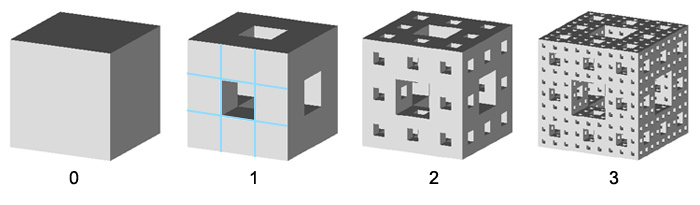
\includegraphics[scale=0.5]{images/cube_fractal.jpg}
\end{center}
\end{problem}

We observe that the object has been broken in 20 pieces, 
and each piece would need to be scaled by a factor of 3
to obtain the original object. Then,

\[
\boxed{
    D = \frac{\log{N}}{\log{\epsilon}} = \frac{\log{20}}{\log{3}} \approx 2.7268,
}
\]
which is less than 3, as expected.


\begin{problem}{Sensitivity and analytical solution}{problem-label-4}

    Consider the map $x_{n+1} = f(x_n) = (2x_n^{2/3} - 1)^3$ , for $x_n \in [-1, 1]$.

    \begin{enumerate}[(a)]
        \item Show, by iterating two close initial conditions, that this map is chaotic.
        \item Show that $x_n = \cos^3 (2^n \cos^{-1} (x_0^{1/3}))$ is a solution $\forall n$.
    \end{enumerate}

\end{problem}

\begin{enumerate}[(a)]
    \item In python, we coded this simple function that implements
    the map and returns the evolution of an initial condition:
    \begin{lstlisting}[style=pythonstyle]
    # Simple function
    def map_evolution(x0: float, iter: int) -> list:
        """
        Computes the evolution of an initial condition.

        Parameters
        ----------
        x0 : float
            Initial condition.
        iter : int
            Number of iterations

        Returns
        -------
        x : list
            Evolution of the initial condition.
        """
        # Add the first element
        x = [x0]

        # Iteration process
        for i in range(iter + 1):
            
            # Compute next element
            next = (2 * x[i] - 1)**3

            # Save
            x.append(next)

        return x
    \end{lstlisting}

    Then we just chose two \textit{extremely} close initial conditions
    and found the evolution of both:
    \begin{lstlisting}[style=pythonstyle]
    # Initial conditions
    x0 = 0.9999999998
    x1 = 0.9999999999

    # Iterate!
    x0_results = map_evolution(x0, iter = 14)
    x1_results = map_evolution(x1, iter = 14)
    \end{lstlisting}

    % Figure
    \begin{center}
        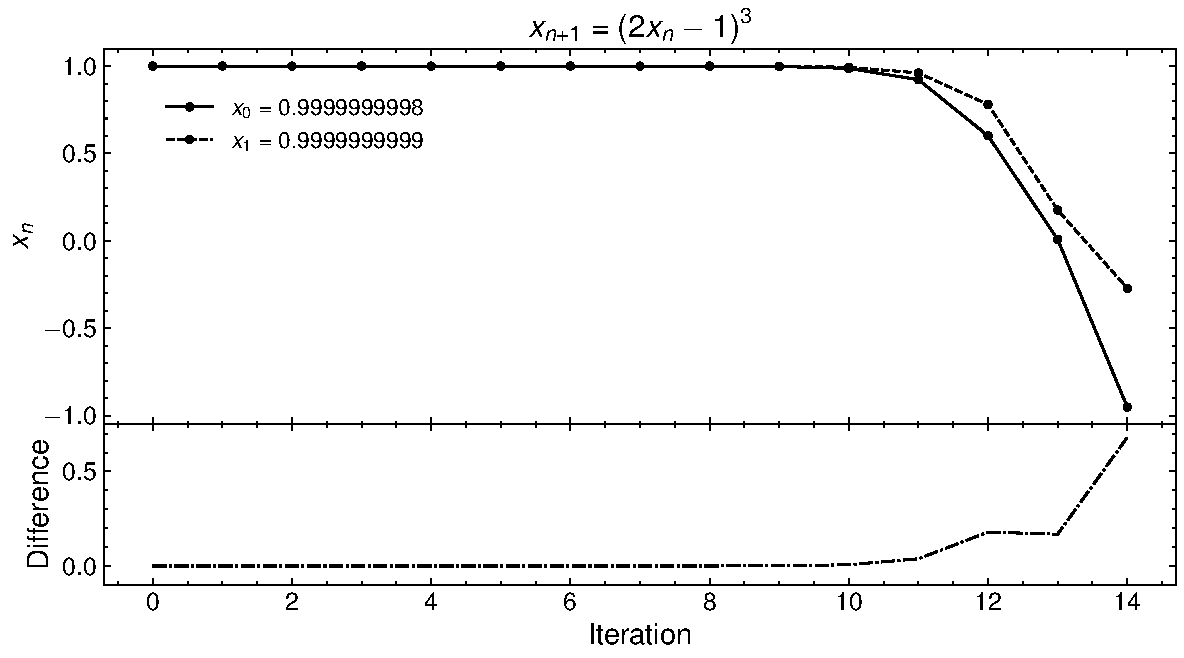
\includegraphics[scale=0.7]{images/4a.pdf}
        \captionof{figure}{Evolution of two close initial conditions, plus
        the difference between them.}
        \label{fig:4a}
    \end{center}

    The results can be seen in figure \ref{fig:4a}. They evolve together
    for the first 10 iterations, but, in the 11th iteration, they start to separate. 
    It takes no time for them to do so, even though they were very close
    at the beginning. \boxed{\text{This is a clear sign of chaos.}}


    \item We'll do it by induction, starting by plugging the expression in the map
    \[
        x_{n+1} = [2(\cos^3 (2^n \cos^{-1} (x_0^{1/3}))^{2/3} - 1]^3.
    \]
    Then, some straightforward algebra gives us
    \[
    \begin{aligned}
        x_{n+1} &= [2\cos^2 (2^n \cos^{-1} (x_0^{1/3})) - 1]^3\\
        &= [2\cos^2 (2\cdot 2^{n-1} \cos^{-1} (x_0^{1/3})) - 1]^3.
    \end{aligned}
    \]
    We can now apply the identity $\cos^2(2x)=(1+\cos(4x))/2$,
    resulting in
    \[
    \begin{aligned}
        x_{n+1} &= \left[2\cdot\frac{1 + \cos(2^2\cdot 2^{n-1} \cos^{-1} (x_0^{1/3}))}{2}-1\right]^3\\
        &= \left[\cos(2^{n+1} \cos^{-1} (x_0^{1/3}))\right]^3\\
        &= \cos^3 (2^{n+1} \cos^{-1} (x_0^{1/3})).
    \end{aligned}
    \]
    Thus, the expression holds for $n+1$. To finish, let's verify the base case
    \[
        x_0 = \cos^3 (2^0 \cos^{-1} (x_0^{1/3})) = \cos^3 (\cos^{-1} (x_0^{1/3})) = x_0^{3/3} = x_0.
    \]

    \boxed{
        \text{Therefore, } x_n = \cos^3 (2^n \cos^{-1} (x_0^{1/3})) \text{ is a solution } \forall n.
    }

\end{enumerate}

\begin{problem}{Bifurcation diagram and Lyapunov exponent}{problem-label-5}
    Consider the map $x_{n+1} = f(x_n) = \sin^2(r\,\arcsin{\sqrt{x_n}})$, for $x_n \in [0, 1]$.

    \begin{enumerate}[(a)]
        \item Obtain the bifurcation diagram of $x_n$ as a function of $r$,
        for $r \in [1, 4]$.
        \item Calculate the Lyapunov exponent as a function of $r$, for $r \in [1, 4]$.
    \end{enumerate}

\end{problem}

Solution goes here.

\begin{problem}{Phase space}{problem-label-6}

    The evolution of a system is described by the following equation:
    \[
        \ddot{x} + a\ddot{x}+\dot{x}-|x|+1=0, \text{ for } a > 0.
    \]

    \begin{enumerate}[(a)]
        \item Find the fixed points of this system.
        \item Plot the attractor of this system in its phase space for $a = 0.6$.
        Is it strange?
        \item Show that this system is not chaotic for $a = 0.68$.
    \end{enumerate}

\end{problem}

Solution goes here.

% Now, let's see how to use the \texttt{problem} environment. 
% The \texttt{problem} environment is defined in the \texttt{format.tex} file. 
% You can define your own environments following 
% the \texttt{problem} environment.

% What do you think about this? I think it's a great 
% way to work with problems. You can also use 
% the \texttt{problem} environment to write your own problems. 
% For instance, you can write your own problems 
% in the \texttt{problem} environment and then use 
% the \texttt{problem} environment to write your own solutions.


% Take this cool equation for example:
% \begin{equation}
%     \label{eq:example}
%     \begin{aligned}
%         \im \hbar \pdv{\psi}{t} &= -\dfrac{\hbar^2}{2m} \nabla^2 \psi + V(x) \psi,
%     \end{aligned}
% \end{equation}

% where $\psi$ is the wave function, $V(x)$ is the potential energy, 
% and $m$ is the mass of the particle. 
% The equation describes how the wave function evolves over time.
% The \texttt{problem} environment is defined in the \texttt{format.tex} file. 
% You can define your own environments following 
% the \texttt{problem} environment.

\vspace{5ex}
\hrule
\vspace{1ex}

\vspace{0.1ex}

% =================================================

% \newpage

% \vfill

% \bibliographystyle{apalike}
% \bibliography{references}

\end{document}